% Тут используется класс, установленный на сервере Papeeria. На случай, если
% текст понадобится редактировать где-то в другом месте, рядом лежит файл matmex-diploma-custom.cls
% который в момент своего создания был идентичен классу, установленному на сервере.
% Для того, чтобы им воспользоваться, замените matmex-diploma на matmex-diploma-custom
% Если вы работаете исключительно в Papeeria то мы настоятельно рекомендуем пользоваться
% классом matmex-diploma, поскольку он будет автоматически обновляться по мере внесения корректив
%

% По умолчанию используется шрифт 14 размера. Если нужен 12-й шрифт, уберите опцию [14pt]
\documentclass[14pt]{matmex-diploma}
%\documentclass{matmex-diploma-custom}
\usepackage{amssymb}
\usepackage{amsmath}
\usepackage{multirow}
\usepackage{graphicx}
\usepackage{subcaption}


\begin{document}
\filltitle{ru}{
    chair              = {Кафедра Системного Программирования},
    title              = {Рандомизированный алгоритм при обработке данных ультразвуковых исследований},
    % Здесь указывается тип работы. Возможные значения:
    %   coursework - Курсовая работа
    %   diploma - Диплом специалиста
    %   master - Диплом магистра
    %    bachelor - Диплом бакалавра
    type               = {bachelor},
    position           = {студента},
    group              = 444,
    author             = {Сенин Иван Игоревич},
    supervisorPosition = {д.\,ф.-м.\,н., профессор},
    supervisor         = {О.\,Н. Граничин},
    reviewerPosition   = {аспирант},
    reviewer           = {К.\,И. Тюшев},
    chairHeadPosition  = {д.\,ф.-м.\,н., профессор},
    chairHead          = {А.\,Н. Терехов}
   university         = {Санкт-Петербургский Государственный Университет},
   faculty            = {Математико-механический факультет},
   city               = {Санкт-Петербург},
   year               = {2016}
}
\filltitle{en}{
    chair              = {Department of Software Engineering},
    title              = {Randomised algorighm in ultrasonic investigation precessing},
    author             = {Ivan Senin},
    supervisorPosition = {professor},
    supervisor         = {Oleg Granichin},
    reviewerPosition   = {postgraduate},
    reviewer           = {Kirill Tyushev},
    chairHeadPosition  = {professor},
    chairHead          = {Andrey Terekhov},
    % city              =   {Saint Petersburg}
}
\maketitle
\tableofcontents
% У введения нет номера главы
\setcounter{section}{0}
\section*{Аннотация}
Ультразвуковая томография нашла широкое применение в медицинской практике. По мере развития технологий стало возможным использование большего количества датчиков для получения более качественного изображения. Кроме того, для хорошей фокусировки необходима высокая частота дискретизации получаемого сигнала, что ведёт к большому объему обрабатываемой информации.  Однако, характер получаемых при томографии изображений имеет разреженный профиль, из чего следует, что необходимое для восстановления количество информации очень мало. В то же время имеется значительная избыточность данных, что оставляет возможность для разработки более оптимальной технологии сбора и анализа в процессе томографического исследования. В этой работе предложен прототип эффективной технологии по сбору и реконструкции изображений ультразвуковой томографии, основанной на принципах рандомизированных алгоритмов, которая позволяет сократить время исследования без потерь в качестве. 


\section{Введение}

\subsection{Актуальность}
Ультразвуковая томография по качеству и разрешающей способности достигла сопоставимого с МРТ уровня и активно применяется для исследования мягких тканей \cite{hopp2014breast}. 
Преимуществами УЗИ являются относительно низкая стоимость оборудования и обслуживания, безопасность для организма, неинвазивность техники исследования. \\
Для повышения качества и разрешающей способности получаемого в ходе исследования изображения требуется увеличение количества используемых датчиков и частоты дискретизации сигнала. Всё это ведёт к значительному увеличению объема передаваемых данных, что усложняет как производственный процесс, так и проведение диагностики. Кроме того особенности проведения исследования допускают наличие помех и искажений \cite{shannon_th}. \\
Опухоли преимущественно имеют более высокую скорость прохождения ультразвука, чем окружающие ткани. Это делает возможным реконструкцию плотностей тканей в исследуемой зоне с помощью уравнений с участием предполагаемых путей распространения сигнала и временем его прибытия на датчики кругового массива (\textit{travel time tomography}) \cite{quan2007sound}. Современные системы основаны именно на таком подходе и получили применение в диагностике рака молочных желез \cite{hormati2010robust}\cite{schreiman1984ultrasound}. \\
Для метода томографии travel-time типична квадратичная от числа сенсоров зависимость получаемых "сырых" данных для анализа: последовательно с каждого датчика пускается ультразвуковой импульс, который принимают остальные $k-1$ сенсоров. Это приводит к серьезному повышению требований к вычислительной части устройства томографа, а также к увеличению времени обработки: современные методы реконструкции работают итеративно с временной сложностью итерации $O(N\log N)$ \cite{chen2012compressive}.


\subsection{Обзор литературы и ключевые работы в области}

\subsubsection{Travel-time томография}
Техника томографии по времени прибытия сигнала уже хорошо изучена и освещена в работах \cite{Kunyansky2012111}, \cite{quan2007sound}, \cite{hopp2014breast}. В том числе рассмотрены алгоритмы в отношении устойчивости к присутствию шума \cite{hormati2010robust}. Далеко не последнюю роль в реконструкции изображения играет точное определение времени прибытия сигнала \cite{li2009improved}. Общий процесс обработки данных томографии времени прибытия показан на рис.\ref{fig:us_process} \\

\begin{figure}[h]
\centering
    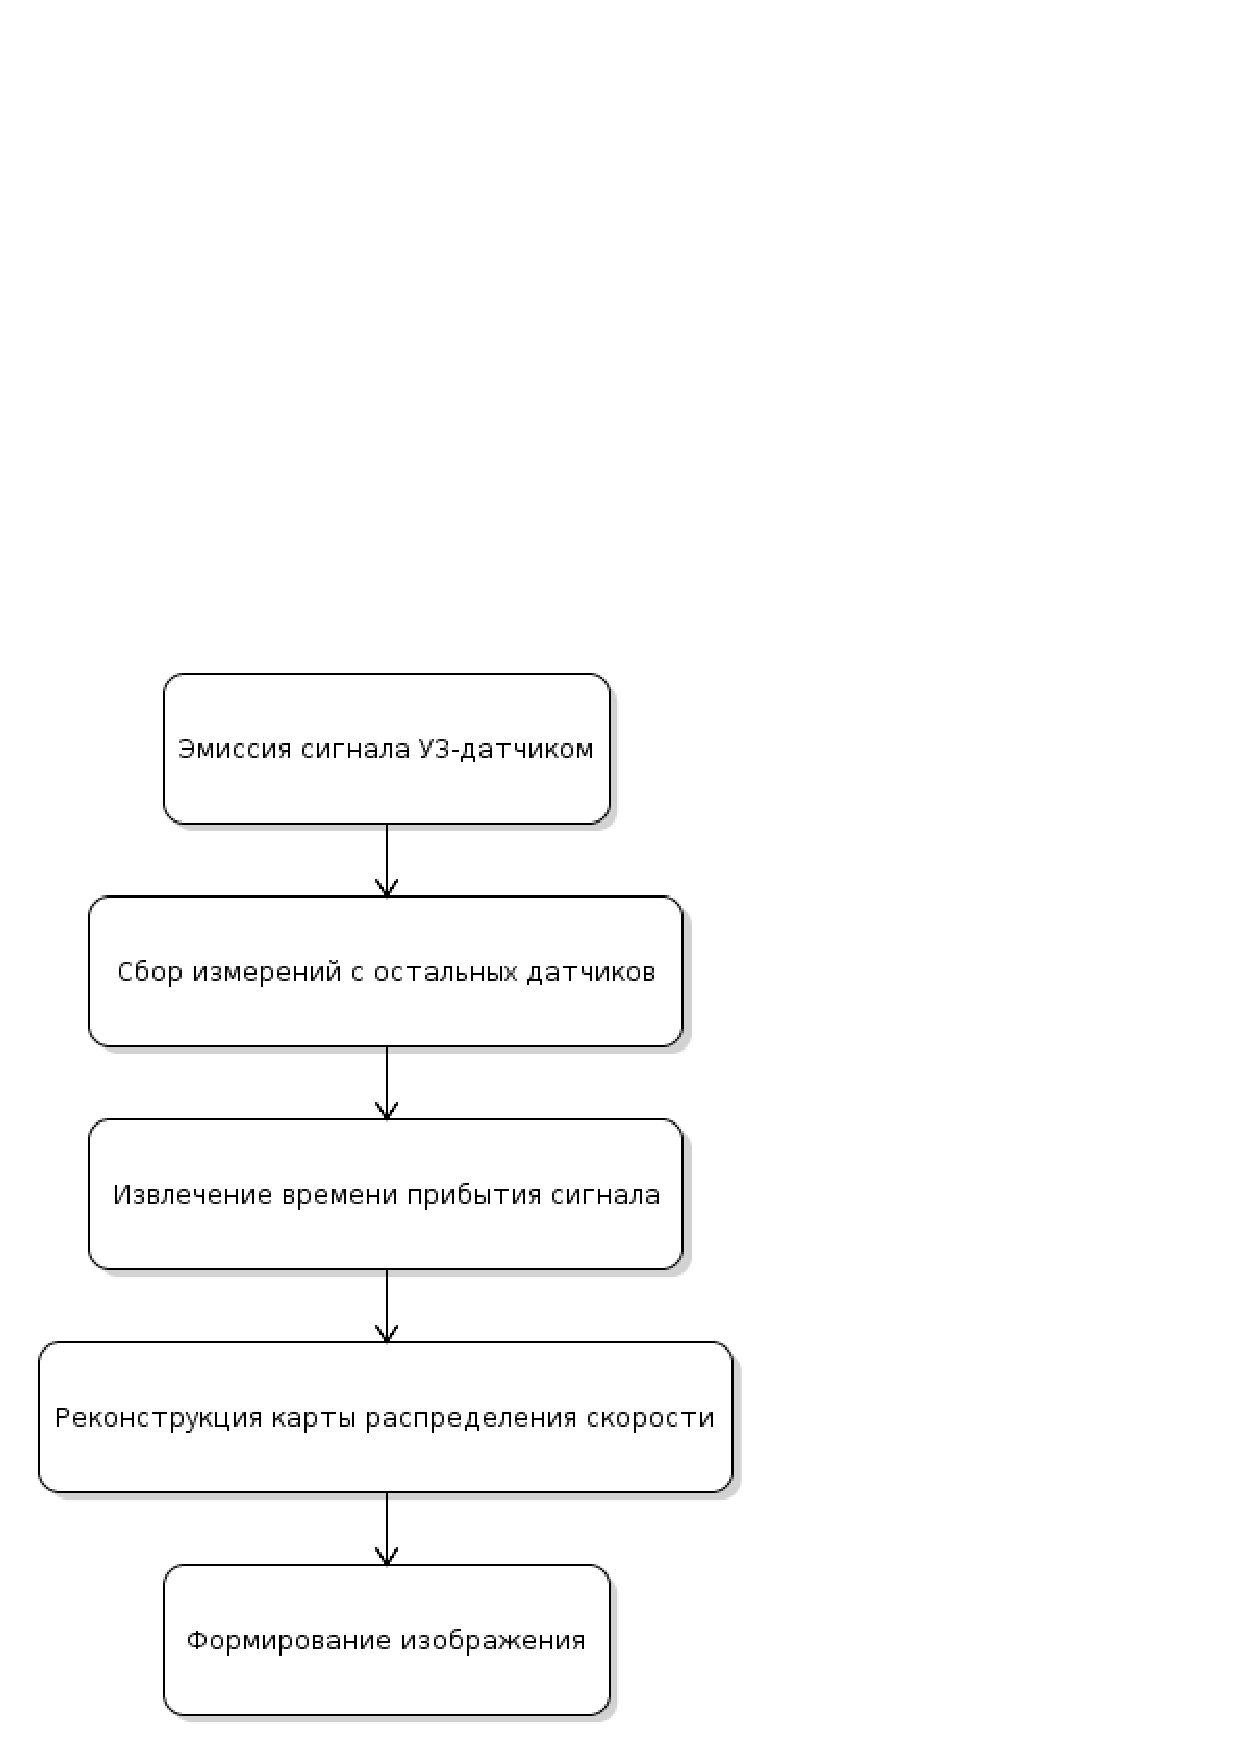
\includegraphics[width=0.5\textwidth]{pics/us_process.png}
	\caption{Общий вид процесса ультразвуковой томографии времени прибытия}
	\label{fig:us_process}
\end{figure}


Основная цель акустической томографии -- восстановить параметры неизвестной среды изучая характеристики распространения звука в ней. Во-первых, для этого требуется точная модель, хорошо описывающая лежащую в её основе физическую систему, и, во-вторых, высокоточные измерения. Тогда решением обратной задачи составляется оценка неизвестной модели. Корректность физической модели, точность измерений и выбор метода решения обратной задачи имеют прямое влияние на качество реконструкции. \\
Распространение энергии акустического сигнала в неоднородной среде хорошо описывается дифференциальным уравнением в частных производных второго порядка 
$$\nabla^2p(r,t) - \frac{1}{F^2(r)}\frac{\partial^2p(r,t)}{\partial t^2} = s(r,t)$$
где $p(r, t)$ --давление в $r$ в момент времени $t$, $F(r)$ -- неизвестная модель распространения скорости и $s(r,t)$ -- первоначальный сигнал. Зная исходный сигнал $s(r, t)$, решая обратную задачу, находим модель $F(r)$, которая лучше всего описывает измерения $p(r,t)|_{\Omega}$, записанные на известных границах $\Omega$.\\
Моделирование прямой задачи по уравнению распространения волны вычислительно весьма трудоёмко, вследствие чего в travel-time томографии используются принципы геометрической акустики. При предположении, что частота звукового сигнала достаточно высока, можно найти его путь распространения используя принципы Ферма \cite{schuster1904introduction}. Тогда обратная задача состоит в реконструкции распределения скорости звука $F(r)$ исходя из времени сигнала в пути, получаемое с показаний датчиков. Следует отметить, что в отличии от задач томографии с помощью рентгена, где сигнал распространяется по прямой, распространение ультразвукового сигнала в неоднородной среде происходит иначе и зависит от распределения скорости.\\
В то время как акустическая \textit{томография по времени прибытия сигнала берет свои корни из сейсмологии}\cite{dines1979computerized}, на сегодняшний день уже множество исследований показало, что ультразвуковая томография имеет большой потенциал в области диагностирования рака груди \cite{duric2007detection}. \\

\textbf{Постановка обратной задачи по реконструкции изображения}\\
Время сигнала в пути от передатчика к приемнику вдоль траектории его распространения можно представить как 
\begin{equation}\label{eq:time_of_fl_cont}
Y = \int_\Gamma \frac{1}{F(r)}ds,
\end{equation}
где $Y$ -- время прибытия сигнала, $\Gamma$ -- путь его распространения, $F(r)$ -- скорость звука в точке $r$. Следует заметить, что проходимый сигналом путь $\Gamma$ зависит от распределения скорости в среде $F(r)$. Существует нелинейная зависимость между временем сигнала в пути и скоростью звука в среде. Можно представить уравнение \eqref{eq:time_of_fl_cont} в дискретной форме, наложив сетку на интересующую для восстановления область с константными значениями скорости звука в клетках общим количеством $N$ ячеек:
\begin{equation}\label{eq:2}
Y = A(F)\cdot F,
\end{equation}
где $F$ -- вектор $[N\times 1]$, представляющий интересующее распределение скоростей, а $A(F)$ -- матрица $[M\times N]$, представляющая путь, по которому проходит сигнал и $t$ -- вектор $[M\times 1]$, содержащий время прибытия сигнала, полученное анализом показаний с датчиков. Так имея в установке $k$ датчиков, получаем $M = k\cdot (k-1)$ всевозможных траекторий кратчайшего прохождения сигнала. \\
Целью обратной задачи является нахождения такой оценки распределения скоростей \^{m}, которая лучше всего описывает время прохождения пути сигналом в уравнении \eqref{eq:2}. Одним из традиционных алгоритмов решения является метод сопряженных градиентов с $\ell_1$ регуляризатором \cite{hormati2010robust}. Тогда задача представляется как задача минимизации
\begin{equation}
\label{eq:lasso}
\min_F \| A(F) \cdot F - Y \|_2^2 + \lambda \| \Psi^T F \|_1,
\end{equation}
где $\Psi$ -- некоторый базис, переводящий $F$ в разреженное представление и $\lambda$ -- некоторый положительный весовой коэффициент. 



\subsubsection{Compressive Sensing}
С начала второго тысячелетия объемы получаемой и обрабатываемой информации существенно возросли. Главным образом это связано с увеличением размерностей передаваемых сигналов (от одномерных "1-D" к дву- и  трех- мерным). При этом рост данных происходит по экспоненциальному закону относительно размерности. Также в современных системах происходит постоянный пост требований к частоте измерений (теорема Шеннона-Найквиста-Котельникова). Всё это влечет необходимость сжатия данных для хранения и пересылки, стоимость суммарной обработки оказывается очень дорогостоящей.
Интересующую информацию можно представить как $x \in \mathbb{X}$, которую предстоит получить с помощью набора наблюдений $y \in \mathbb{Y}$. Между $x$ и $y$ существует закономерность явления $\Phi:\mathbb{X}\to\mathbb{Y}$. В случае, когда $\Phi$ обратим и при линейной зависимости, известно, что $x = \Phi^{-1}y $. Для систем реального мира более типичным является случай, когда результаты наблюдений подвержены различным помехам \[y = \Phi x + \xi\] 
При значительных помехах задача решается статистически, используя $m >> N$ при $x \in \mathbb{R}^N$. Известно, что такая задача о восстановлении $x$ может быть решена даже в случае нецентрированных коррелированных помех за счет случайного выбора матрицы $\Phi$ \cite{granichin2004linear}. Установлено, что рандомизация позволяет не только устранить эффект смещения, но и уменьшить количество итераций алгоритма оценивания $x$ \cite{граничин2003рандомизированные}. \\
На практике интересно рассмотреть возможности восстановниея $x \in \mathbb{R}^N$ при $m << N$, что, очевидно, невозможно в общем случае. Однако, оказалось, что задача может быть решена с достаточной точностью, при выполнении некоторых условий \cite{donoho2006compressed}. Подобная парадигма получения и восстановления данных называется \textit{Compressive Sensing} или \textit{Опознание со сжатием}. \\
Постановка задачи о получении и восстановлении данных в общем виде выглядит следующим образом. Пусть $x$ -- интересующая информация. Она проявляется себя через сигнал $f = \Psi x$. С помощью каких-либо приборов регистрирования получают наблюдения $y = A f$. По ним исследователю необходимо восстановить исходную информацию $x$, формируя оценки \^{x}. \\
\textbf{Проектирование матрицы измерений}\\
Получение $m < N$ наблюдений можно представить как скалярное произведение с множеством некоторых векторов $\{a_i\}_{i=1}^m$, или умножением на матрицу размерности $m\times N$: $y= A f$. Тогда из постановки задачи следует $y=A f = A \Psi x = \Phi x$, где $\Phi$ - матрица $m \times N$. \\
Необходимыми и достаточными условиями, предъявляемыми теорией \textit{опознания со сжатием}, являются: 
\begin{itemize}
\item сигнал $f$ является $s-$разреженным: \\существует такой базис $\Psi$, что $f = \sum_{j=1}^N x[j] \psi_j$, где только $s$ коэффициентов $x[j]\neq 0$
\item выполняется "свойство ограниченной изометрии" (Restricted Isometry Property, RIP):
$$\text{RIP}(\delta, m)= \sqrt{1 - \delta} \leq \frac{\| \Phi z \|_2}{\| z\|_2} \leq \sqrt{1 + \delta}$$, где $\delta \in (0,1)$ и $z$ - произвольный ненулевой $m-$разреженный вектор

\item свойство "некогерентности" (малой взаимной зависимости) $A$ и $\Psi$: 
$$\mu (A, \Psi) = \sqrt{N} \max_{i,j}\frac{|\langle a_i, \psi_j\rangle |}{\| a_i\|_2}$$
Установлено, что случайные матрицы $A$ с высокой вероятностью некогерентны с любым фиксированным базисом $\Psi$.
Из \cite{candes2007sparsity} следует достаточное условие для высокой вероятности точного восстановления $s-$разреженных векторов по m наблюдениям: 
\begin{equation}m \geq c \mu (A,\Psi)^2 s \log{N}, \end{equation}
где $c$ --- некоторая положительная постоянная.
\end{itemize}
В \cite{cande2008introduction} указывается замечание, что на практике часто достаточно $m\approx 4s$. Также известно, что условие $\text{RIP}(\delta, 2s)$ является недостаточным для восстановления в присутствии помех или если в сжимаемом сигнале $N - s$ компоненты малы, но не равно нулю. Для робастности же достаточным условием будет $\text{RIP}(\delta, 3s)$. Явное построение матрицы измерений $A$: $\Phi = A\Psi$ требует проверки условия RIP для каждой комбинации положений $s$ ненулевых компонент вектора $z$ длиной $N$ (т.е. $C_N^s$). Однако, оказывается, что случайная матрица $m \times N$ с элементами $a[i, j] \sim \mathcal{N}(0, \frac{1}{m})$ имеет следующие полезные свойства\cite{candes2006robust}:
\begin{itemize}
\item если $m \geq c_1 s \log{\frac{N}{s}}$ при $0 < \delta < 1$, тогда \\ 
$$\mathcal{P}\{A \in \text{RIP}(\delta, m)\} \geq 1 - 2e^{-c_2 m},$$где $\mathcal{P}$ -- вероятность и $c_1,c_2 > 0$  -- малые постоянные, зависящие от $\delta$. И тогда, следовательно, $s-$разреженные сигналы длины $N$ могут быть восстановлены по $m << N$ измерениям с высокой вероятностью. 
\item если матрица $A$, удовлетворяет указанным условиям, то и $\Phi = A\Psi$ также будет являться матрицей с независимо нормально-распределенными элементами, что влечет $\Phi \in \text{RIP}(\delta ,m)$ с той же вероятностью и для любого ортонормированного базиса $\Psi$
\end{itemize}
Для использования опознания со сжатием помимо проектирования матрицы измерений $A$ требуется разработать \textbf{алгоритм реконструкции сигнала}, задачей которого восстановить по $y \in \mathbb{R}^m$, матрице измерений $A$ и базису $\Psi$ сигнал $f \in \mathbb{R}^N$, или эквивалентное ему спектральное разреженное представление $x$.\\
При $m < N$ для $s-$разреженных сигналов имеется бесконечное число $x'$ : $\Phi x' = y$, т.к. если $\Phi x = y \implies \Phi(X+r) = y$ для любого $r \in \text{Ker }\Phi$. Таким образом, алгоритм реконструкции должен найти вектор разреженного представления сигнала в $(N - m)$-размерном подпространстве $\mathcal{H}=\text{Ker }\Phi + x$.\\
\textbf{Методы решения обратной задачи}\\
Традиционным подходом в решении подобных обратных задач является поиск в $\mathcal{H}$ вектора с минимальной энергией (нормой)  $\ell_2$: $$ \hat{x} = \arg\!\min{\| x'\|_2} : \Phi x' = y$$, или, что тоже самое, в форме метода наименьших квадратов 
$$\hat{x} = \Phi^T (\Phi\Phi^t)^{-1}y$$
Поскольку $\ell_2$ норма  отражает энергию сигнала, а не разреженность, результат будет содержать много ненулевых компонент. С задачей поиска разреженного решения хорошо справляется "$\ell_0-$норма". Однако, задача $\ell_0$ оптимизации невыпукла и относится к комбинаторному типу, процедуры ее решения, в общем случае, $NP-$сложные \cite{natarajan1995sparse}. Существует два подхода для приближенного решения таких задач: "жадные" стратегии оптимизации\cite{mallat1993matching} или переход к $\ell_1-$норме. Хорошо известно, что минимизация $\ell_1$ нормы способствует разреженности \cite{donoho2006most} и позволяет хорошо приближать разреженные сигналы используя только $m \geq c_1 s \log{\frac{N}{s}}$ случайных измерений \cite{donoho2006compressed}\cite{candes2006robust}. Это задача выпуклой оптимизации, сводимая к известной задаче линейного программирования "выбор базиса" (Basis Pursuit De-noising) \cite{chen2001atomic}, эффективные методы решения которого имеют временную сложность $\mathcal{O}(N\log{N/s})$ \cite{berinde2008practical}.




Техника обработки сигналов \textit{Compressive Sensing} может быть использована для решения проблемы передачи и обработки большого количества информации с массива датчиков. Этот метод уже успешно применяется в магнитно-резонансной томографии \cite{lustig2008compressed}\cite{lustig2007sparse}.







\subsection{Предварительный пример}
В целях получения наилучшего изображния требуется большое количество датчиков и высокая частота дискретизации сигнала. Всё это ведёт к необходимости обработки серьезного объема данных. Оценить количество данных, поступающих непосредственно с датчиков можно как
\[ V = k^2  z  Y_{max} \nu,   \]
где $V$ --- общее число измерений сигнала, $k$ --- количество датчиков, $z$ --- количество исследуемых срезов, $Y_{max}$ --- время прохождения сигнала с учетом затухания эха, $\nu$ --- частота дискретизации. \\

Примером современного коммерческого ультразвукового томографа является The SoftVue\cite{roy2013breast}, который имеет следующие технические характеристики системы:
\begin{itemize}
\item Мастер сервер: 2 процессора quad-core Intel Xeon E5620, 192 ГБ ОЗУ
\item Сервер реконструкции: 2 процессора quad-core Intel Xeon E5620, 96 ГБ ОЗУ, 2 ГП Nvidia Tesla M2070
\end{itemize}
Так в таблице \ref{table:datasize_ex} производители описали количество данных, получаемоых с датчиков за один срез. На обработку такого среза при использовании только одного сервера для реконструкции требуется несколько минут\cite{roy2013breast}.


\begin{table}
\centering
\caption{Объем исходных данных ГБ за один срез в зависимости от числа датчиков в массиве и частоты дискретизации сигнала \cite{roy2013breast}}
\begin{tabular}{ c | c | c | c }
    \hline
    \multirow{2}{*}{Частота дискретизации (МГц)} & \multicolumn{3}{c}{Число датчиков}  \\ \cline{2-4}
    & 256 & 51 & 1024 \\
    
    \hline
    10 & 0.21 & 0.86 & 3.44 \\
    12 & 0.26 & 1.03 & 4.13 \\
    14 & 0.30 & 1.20 & 4.81 \\
    \hline
\end{tabular}

\label{table:datasize_ex}
\end{table}




\subsection{Требования к системе}
\textit{TODO: Требования, которые мы предъявляем к нашей технологии или к технологии сбора и обработки данных?} \\
\\
Традиционный способ сбора и обработки данных можно существенно улучшить, получив выигрыш по времени, как затрачиваемым на реконструкцию изображения, так и на непосредственно исследование пациента.

\subsection{Основной результат (обзор)}
\textit{TODO: разработана "технология", что на вход идут характеристики прибора и результаты симуляции, а на выходе получаем все необходимые параметры для рандомизированного алгоритма} \\
\\
Разработан метод, позволяющий при разработке ультразвукового томографа эффективно внедрить в применяемые алгоритмы по сбору и обработке данных парадигмы опознания со сжатием, способной существенно снизить требования к вычислительным мощностям прибора. Эксперименты, проведенные на полноразмерной компьютерной модели, показали сокращение количества машинных операций, затраченных на реконструкцию, на N\%. Проведено аппробирование на прототипе ультразвукового томографа, результаты которого свидетельствуют об уменьшении размера "сырых" данных на X\%. 

\subsection{Структура работы}
\textit{TODO: forward} \\

\section{Постановка задачи}
\subsection{Цель работы}
\textit{TODO: неформальное описание технологии с точки зрения пользователя} \\
\begin{itemize}
  \item Разработать прототип технологии по сбору данных и реконструкции изображения с различных проекций устройства ультразвуковой томографии
  \item Разработать рандомизированный алгоритм для сбора и передачи данных ультразвуковой томографии. Алгоритм должен быть пригоден для обработки данных, полученных на устройстве ультразвуковой томографии, использующем 1024 датчика.  
  \item Методом программной симуляции выяснить характеристики полученного алгоритма. В частности, выяснить минимальное число собираемых проекций для реконструкции приемлемого качества
\end{itemize}

\subsection{Постановка задачи}
\textit{TODO: Цели по порядку с точки зрения математики} \\
\begin{itemize}
\item определить необходимое количество измерений
\item спроектировать матрицу $A'$
\item разработать алгоритм восстановления "сигнала"
\end{itemize}



\section{Основной результат}


\subsection{Исследование разреженности изображения}

\textbf{Выбор метрики для пространства карты скоростей $F$} \\
\textit{Привести аргументированное обоснование выбора нормы Фробениуса: сделать исследование или заменить метрику на типично используемую в подобных исследованиях} \\

Для сравнения результатов проведенной реконструкции с исходной моделью, а также, в дальнейшем, результатов, полученных с применением опознания со сжатием, требуется выборать метрику, наилучшим образом описывающую расстояние в пространстве разреженных изображений. 
\begin{description}
\item Метрика относительной ошибки показала неудовлетворительный результат, причиной чего является локальность всплесков скоростей. 
\item Норма Фробениуса $\| F \|_2 = \sqrt{\displaystyle\sum_{i,j}{| a_{ij} |^2}}$ продемонстрировала хороший результат
\end{description}


\subsubsection{Описание маломасштабной модели} \label{sec:model_desc}

Для исследования по внедрению парадигмы опознания со сжатием в сфере ультразвуковой томографии была взята следующая компьютерная\textit{(синоним?)} модель:
\begin{itemize}
\item Диаметр кольца массива датчиков $d = 6 \text{ см}$
\item Полное число датчиков массива, равномерно распределенных по периметру кольца: $k = 100$
\item Число датчиков, используемых для получения сигнала, $k_{Rx} = \frac{1}{3} \cdot k$
\item Сетка реконструкции $N = 64\cdot 64$
\item Число срезов $z_{total} = 15$
\item Модель исследуемой ткани задана двумя объектами, представляющие опухоль со скоростью прохождения звука $f_t = 2600$ м/с. Остальное пространство "заполнено водой" со скоростью звука $f_w = 1500$ м/с. Модель среза $z = 3$ представлена на рис.\textit{(сделать рисунок)}. 

\end{itemize}
\textit{TODO: возможно, следует каким-то образом перенести описание модели в раздел моделирования, но я ниже провожу анализ по результатам, основанным на этой модели}


\subsubsection{Анализ карты скоростей в домене вейвлет-коэффициентов} \label{sec:s_analysis}
Известно, что томографические снимки имеют разреженный характер[?]. К категории эффективных трансформирующих преобразований, позволяющих привести восстановленную карту скоростей $F$ к разреженному представлению, относятся вейвлет-преобразования. Исследования[мои или найти ссылки] показали эффективность вейвлета Добеши D4 в контексте решаемой задачи. \\
На рис.\ref{fig:wavelet_transform} представлен пример использования вейвлета D4, примененного к результату реконструкции среза $z=3$ маломасштабной модели (см. \ref{sec:model_desc}) рис.~\ref{fig:speedmap}. Результат преобразования $X = \Psi^{-1} F$ представлен на рис.~\ref{fig:waveletted}.\\

\begin{figure}[h]

\begin{subfigure}{.5\textwidth}
    \centering
    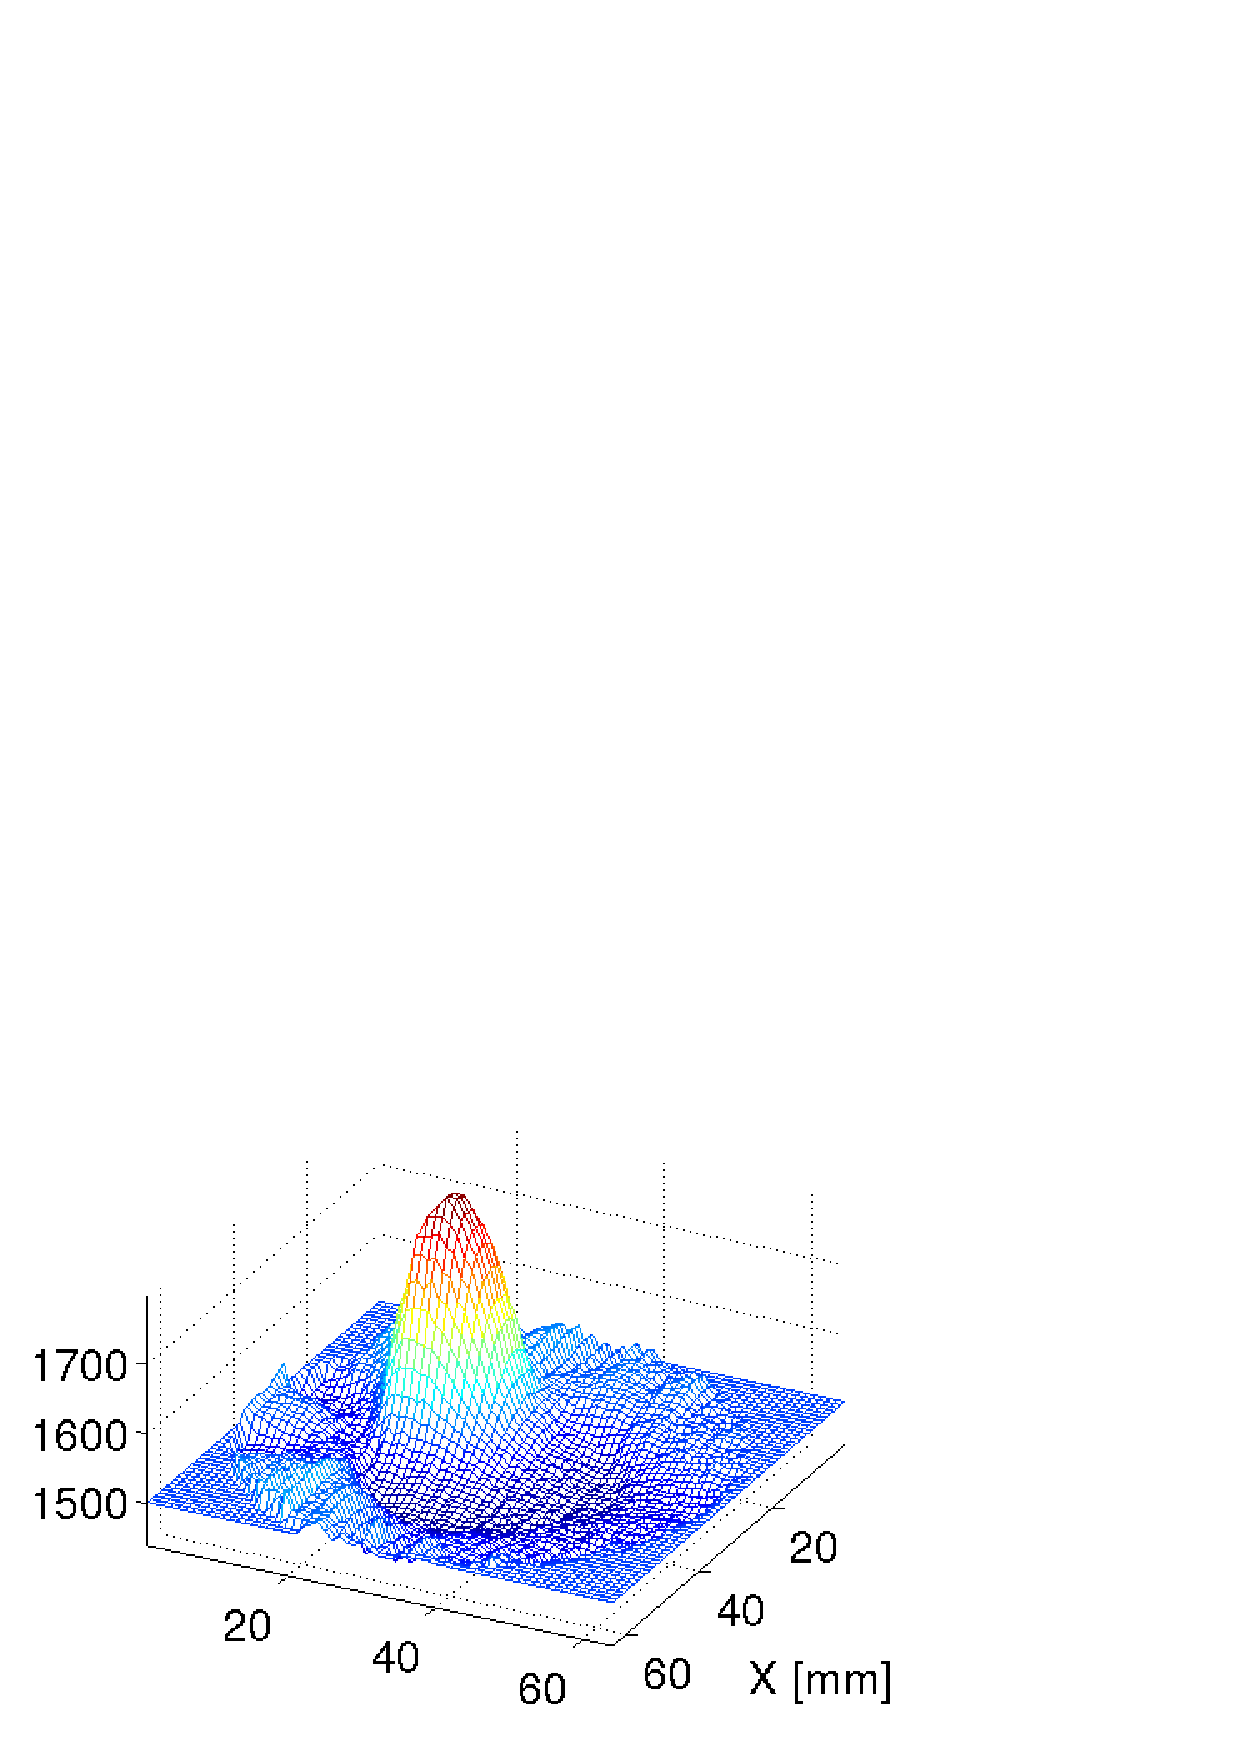
\includegraphics[width=0.8\linewidth]{pics/speed_map.png}
    \caption{Карта скоростей восстановленная из сигнала}
    \label{fig:speedmap}
\end{subfigure}
\begin{subfigure}{.5\textwidth}
    \centering
    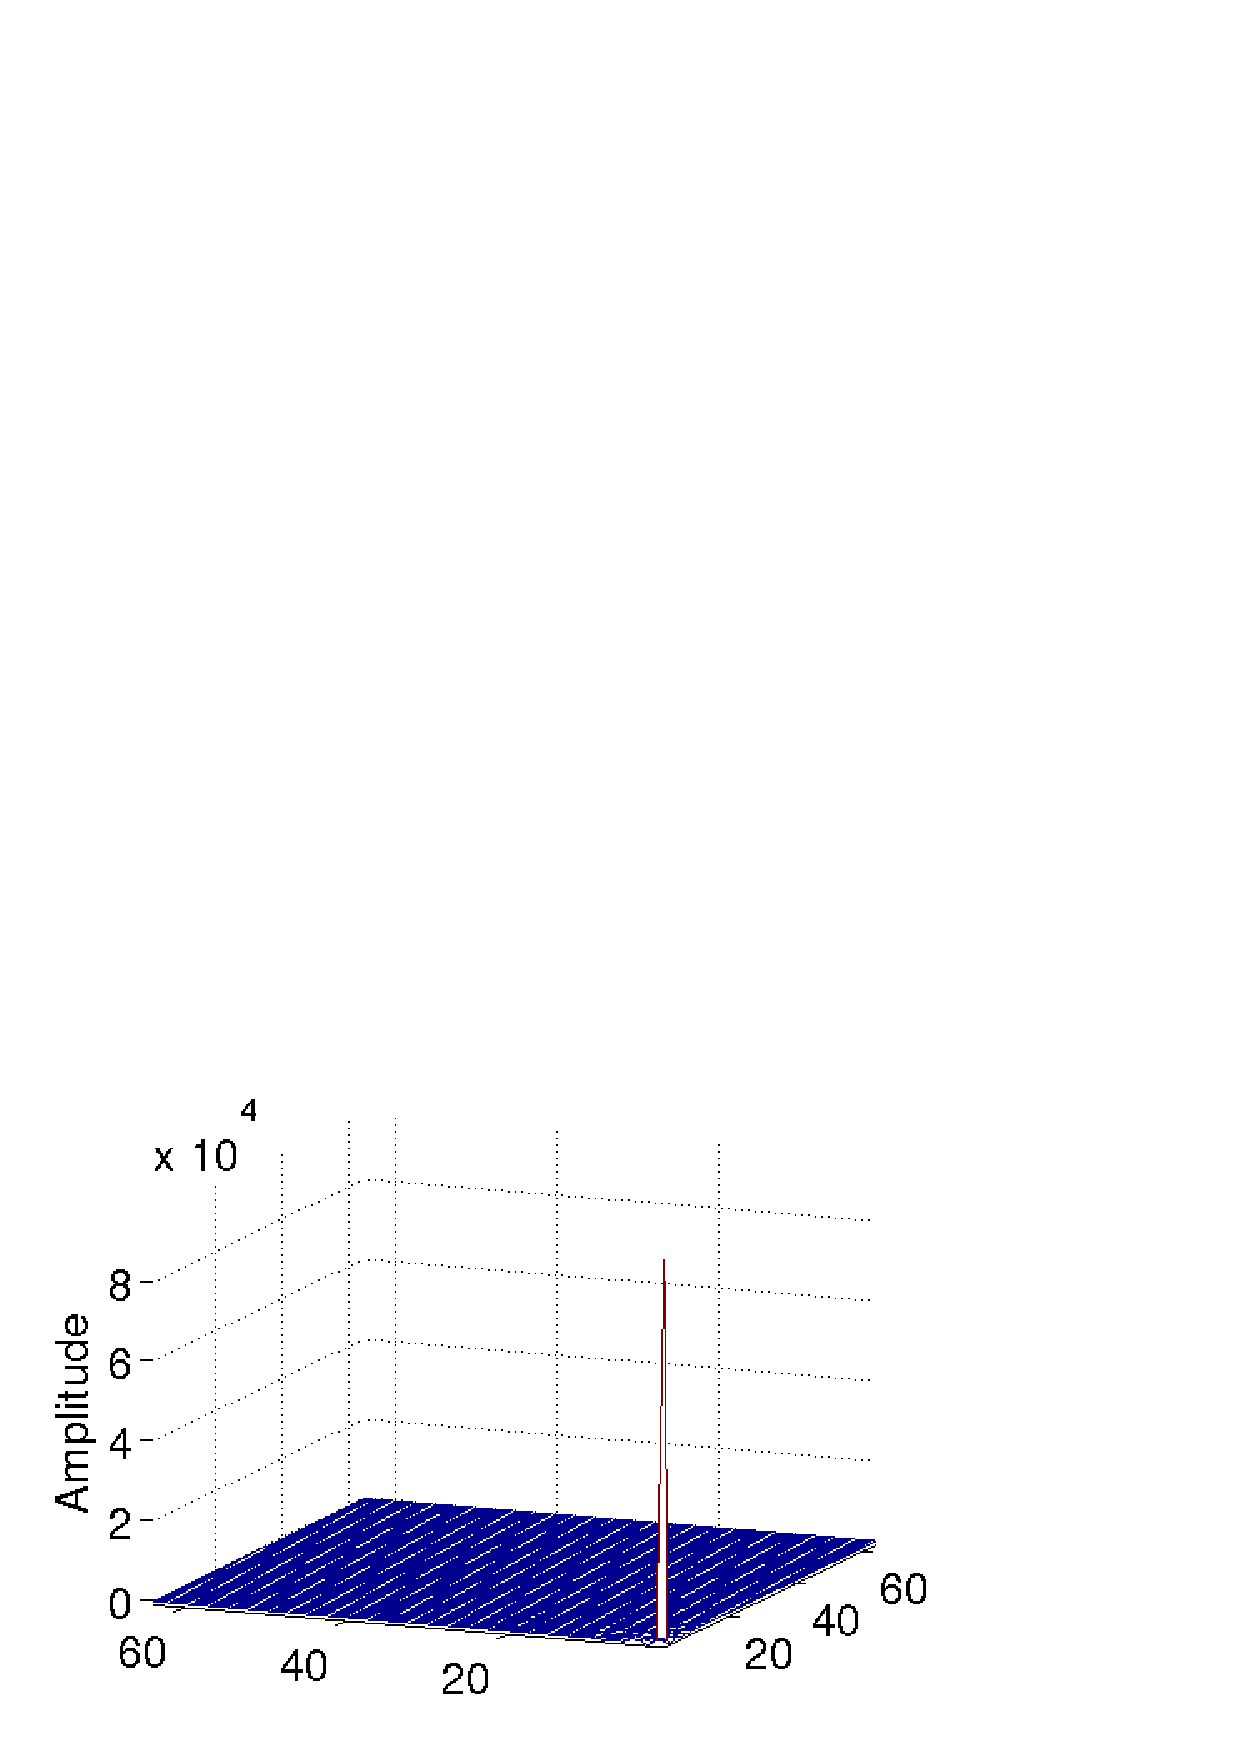
\includegraphics[width=0.8\linewidth]{pics/freq_domain.png}
    \caption{Представление карты скоростей после вейвлет-преобразования}
    \label{fig:waveletted}
\end{subfigure}
	\caption{Вейвлет-преобразование переводит карту скоростей в разреженное представление}
	\label{fig:wavelet_transform}
\end{figure}

\textit{TODO: Возможно добавить результат вейвлет-обработки для взятого-откуда-нибудь типичного томографического снимка} \\

Согласно маломасштабной модели, общее количество коэффициентов составляет $N = 4096$.  Легко убедиться в разреженности сигнала: рис.~\ref{fig:used_coeff} демонстрирует, что при использовании только лишь 100-200 коэффициентов происходит восстановление близкое к полному. \\

\begin{figure}[h]
\centering
    \includegraphics[width=1\textwidth]{pics/used_coeff.png}
	\caption{Ошибка восстановления карты плотностей при использовании неполного набора коэффициентов вейвлет разложения}
	\label{fig:used_coeff}
\end{figure}

Это означает, что, в контексте опознания со сжатием, характеристику сигнала $s$ для маломасштабной модели можно выбрать на промежутке от 100 до 200. В дальнейшем будем полагать $s=13^2 = 196 $.




\subsection{Проектирования рандомизированной матрицы}
\textit{TODO: Обоснование, что случайный выбор датчиков будет удовлетворять критериям CS}\\


\subsection{Процесс реконструкции при применении CS}
\textit{TODO: $\ell_1$ минимизация заложена в эффективный метод решения обратной задачи LASSO (см. уравнение \eqref{eq:lasso})}\\

\subsection{Ожидания по масштабированию задачи}
Общее число уравнений, получаемых в результате максимально возможного числа проекций томографического обследования, \[M = k\cdot (k-1),\] где $k$ - количество датчиков в массиве устройства. 
Полезным результатом теории опознания со сжатием является тот факт, что единожды установив характеристику $s$, можно проводить масштабирование сетки реконструкции $F$ и, не проводя повторных экспериментов, получать необходимое количество используемых уравнений
\begin{equation}\label{eq:approx_m}
m \approx 4 s  \log{\frac{N}{s}} 
\end{equation}
Так по рис.~\ref{fig:percents} видно преимущество, получаемое при использовании парадигмы опознания со сжатием: количество уравнений, необходимых для реконструкции требуемого разрешения, растет логарифмически по сравнению с традиционным способом использования полного набора $M$ уравнений.

\begin{figure}[h]
\centering
    \includegraphics[width=1\textwidth]{pics/percents.png}
	\caption{Процент уравнений, достаточных для реконструкции}
	\label{fig:percents}
\end{figure}



\subsection{Описание технологии использования рандомизации как результат работы}
\textit{TODO: Здесь будет описание методики внедрения CS при разработке томографа, всякие UML диаграммы и описание программного комплекса} \\


\section{Моделирование}

\subsection{Результаты применения опознания со сжатием на маломасштабной модели}
\begin{figure}[h]

\begin{subfigure}{.32\textwidth}
    \centering
    \includegraphics[width=1\linewidth]{pics/ref_kwave_30p.png}
    \caption{Изображение, полученное при использовании 30\% данных}
    \label{fig:percents_30}
\end{subfigure}
\begin{subfigure}{.32\textwidth}
    \centering
    \includegraphics[width=1\linewidth]{pics/ref_kwave_70p.png}
    \caption{Изображение, полученное при использовании 70\% данных}
    \label{fig:percents_70}
\end{subfigure}
\begin{subfigure}{.32\textwidth}
    \centering
    \includegraphics[width=1\linewidth]{pics/ref_kwave_99.9p.png}
    \caption{Изображение, полученное при использовании всего объема данных}
    \label{fig:percents_100}
\end{subfigure}

    \caption{Результаты реконструкции при использовании различного объема исходных данных}
    \label{fig:reconstruction_exp1}
\end{figure}

\textit{TODO: улучшить обоснование выбора s; оценить адекватность графика \ref{fig:used_equations} }\\
Для эксперимента по применению опознанию со сжатием была использована следующая модель:
\begin{itemize}
\item Исследуемая область заполнена водой. В центр помещена опухоль диаметром 5 мм
\item Скорость прохождения звука в воде $f_w = 1500$ м/с Скорость прохождения звука через опухоль: $f_t = 2600$ м/с
\item Диаметр кольца массива датчиков $d = 4 \text{ см}$
\item Полное число датчиков массива, равномерно распределенных по периметру кольца: $k = 100$
\item Число датчиков, используемых для получения сигнала, $k_{Rx} = \frac{1}{4} \cdot k$
\item Сетка реконструкции $N = 64\times 64$
\end{itemize}
Для симуляции модели был использован специальный инструмент для ультразвуковых исследований в среде Matlab "K-Wave". K-Wave неоднократно использовался в научных работах [ref].\\
В описанной выше модели для реконструкции можно использовать до $M = k_{Rx} \cdot k^2 = 2500$ уравнений. Повторив анализ, описанный в разделе \ref{sec:s_analysis}, мы находим $s=11^2$. 
Таким образом, применяя уравнение \eqref{eq:approx_m}, получаем достаточное для хорошей реконструкции количество уравнений $m \approx 1700$, что составляет около 68\% от общего их количества $M$. \\
На графике \ref{fig:used_equations} отражена зависимость качества реконструкции изображения от количества исходных данных, где наилучшее значение покателя "отношение сигнал-шум" достигается при использовании 60-75 \% данных. 

\begin{figure}[h]
\centering
    \includegraphics[width=.7\textwidth]{pics/kwave_snr.png}
    \caption{Зависимость качества реконструкции от объема использованных данных относительно исходной модели}
    \label{fig:used_equations}
\end{figure}

Результаты реконструкции при использовании 30, 70 и 100 \% данных представлены на рис.~\ref{fig:reconstruction_exp1}.




\subsection{Расчет и (возможно) результаты для полномасштабной модели с 1024 датчиками}
\textit{TODO: результатов еще нет. Но с использованием CS провести реконструкцию на обычном ноутбуке вполне реально за какое-то разумное время меньше 10 часов. Первые попытки при использовании сетки 64x64 показали, что нужна дополнительная оптимизация для извлечения времени прибытия сигнала с датчиков; неизвестно, нужно ли менять параметр s; }\\

\section{Заключение}
\textit{TODO: Переформулировка из раздела постановки задачи в совершенном виде. Важно написать выигрыш в количественном измерении: ускорили работу алгоритма реконструкции на N\%} \\
\\
\\


% \begin{equation}
% \min_F  \sqrt{\displaystyle\sum_{i=1}^{M} (\displaystyle\sum_{j=1}^N | A_{i,j}F_i - Y_i |^2)}
% + \lambda \displaystyle\sum_{i=1}^N (\displaystyle\sum_{j=1}^N| \Psi_{i,j} F_i|)

% \end{equation}

% ----------------------------------------------------------------------------------


\setmonofont[Mapping=tex-text]{CMU Typewriter Text}
\bibliographystyle{ugost2008ls}
\bibliography{diploma.bib}
\end{document}
